\documentclass[twoside,a4paper,10pt]{article}
\usepackage[T1]{fontenc}
\usepackage[utf8]{inputenc}
\usepackage[english]{babel}
\usepackage{csquotes}

\usepackage[usenames,dvipsnames]{color}
\usepackage{tikz}
\usepackage{pgfplots}
\usepackage{pgf}
\def\barcolor{red!80!black}
\def\barcolorr{blue!80!white}
\def\bardrawcolor{black}
\def\xticklabel{rotate = 45, anchor = east}

\usepackage{xspace}
\usepackage{graphicx}
\usepackage{parskip}
\usepackage{array}
\usepackage{tabularx}
\usepackage{lscape}
\usepackage{verbatim}
%\definecolor{TGred}{rgb}{.6,0,0}
\usepackage{cleveref}

%\usepackage[style=chicago-notes,autocite=footnote,firstinits=true,backend=bibtex]{biblatex}
\usepackage[style=chicago-notes,backend=bibtex]{biblatex}
\addbibresource{bib.bib}

\usepackage[font=small,font=it,labelsep=endash]{caption}

\usepackage{microtype}

\frenchspacing

\usepackage{enumitem}

\usepackage{appendix}

\usepackage{mparhack}
\def\degree{${}^{\circ}$\xspace}

%\newcommand{\fixme}[1]{{\color{red} #1}}
%\newcommand{\marginfixme}[1]{\marginpar{\raggedright \color{red} #1}}
\usepackage[hmargin=3cm,vmargin=2.5cm]{geometry}

\widowpenalty10000
\clubpenalty10000

\usepackage{placeins}

\usepackage{bibleref}
\def\bv{\bibleverse}
\usepackage{ecjhebrew}
\newcommand{\cl}[2]{\begingroup\beginL\begingroup\color{#1}\beginR#2\endR\endgroup\endL\endgroup}
\newcommand{\hebr}[1]{\cjRL{#1}}

%\usepackage{minted}
%\usepackage{listings}
%\newcommand{\mi}[1]{\lstinline{#1}}
\newcommand{\mi}[1]{\emph{#1}}

\newcommand{\myTitle}{Participants in direct speech\xspace}
\newcommand{\mySubtitle}{A computer-assisted analysis of participant reference and participant tracking in Biblical Hebrew direct speech sections\xspace}
\newcommand{\myDegree}{Master of Arts in Theology\xspace}
\newcommand{\myName}{Grietje Commelin-Troost\xspace}
%\newcommand{\mySupervisor}{prof. dr. W.T. van Peursen\xspace}
\newcommand{\posttitle}{Supervisor: prof. dr. W.T. van Peursen\xspace}

\usepackage{hyperref}

\hypersetup{pdftitle={\myTitle},%
	pdfauthor={\myName},%
	pdfsubject={\myTitle},%
	pdfkeywords={},%
	pdfcreator={pdfLaTeX},%
	pdfproducer={LaTeX},%
	colorlinks,linkcolor=TGred,urlcolor=TGred,citecolor=TGred
}

\raggedbottom

\begin{document}
\pagenumbering{gobble}
\begin{center}
\null
\vspace*{40ex}
{\LARGE \myTitle}\\
\vspace*{10ex}
{\Large \mySubtitle}\\
\vspace*{55ex}
{\large \myName}\\
\bigskip
{\large Promotor: prof. dr. W.T. van Peursen}\\
\bigskip
\normalsize \today
\vfill
\end{center}

\newpage
\newpage
\section*{Abstract}
\newpage
\section*{Samenvatting}
\newpage
\section*{Table of contents}
\newpage
\section*{Abbreviations and key terms}
\subsection{Abbreviations}
\begin{tabbing}
QF \hspace{5ex} \= Quotative Frame \\
DSU \> Direct Speech Unit \\

\end{tabbing}

\subsection{Key terms}
Some key terms that are used in this dissertation, are used by other researchers as well. However, nuances in meaning might differ. Other terms are coined by myself, because existing terms have connotations that would be misleading in my use of them. To avoid confusion, below I give an overview of some key terms.

\begin{tabular}{p{19ex}p{80ex}}
Direct Speech Unit & An uninterrupted portion of direct speech, together with its Quotative Frame. In practice, this often means that a Direct Speech Unit forms one turn in a conversation or a closed-off portion of direct speech within a non-direct speech context. \\
Quotative Frame & The clause(s) immediately preceding a portion of direct speech that introduce this direct speech section. A Quotative Frame usually contains one or more verbs of speech, e.g. \hebr{WJMR} (``he said'').\\
Participant & Any entity playing an active or passive role in a text. The prototype participant is an acting or speaking human person, but non-human and even non-animate entities can also be participants. \\
Participant reference & Any textual designation referring to a participant. A good starting point is to consider any text element that has an encoding for person, number and/or gender as a participant reference.\\
Participant reference system & A language-specific set of ``rules'' about the encoding of participants. \\
Participant tracking & The process of determining which participants are referred to in a text.\\
Verb of speech & Also called ``verb of quotation''. A type of verbs denoting a speech act, and therefore often introducing a portion of direct speech. The verbs of speech that occur in the Hebrew Bible are: \hebr{>MR}, \hebr{DBR}, or (in \bibleverse{Daniel}) \hebr{MLL}.

\end{tabular}

\newpage
\section*{Acknowledgments}
\begin{itemize}
\item Van Peursen
\item Talstra
\item Johan!!!
\end{itemize}
\newpage
\section{Introduction}
\subsection{Topic / problem}
The Hebrew Bible is full of participants acting in narratives, speaking to each other, or being spoken about. Usually, it is pretty clear who is who and what each participant is saying or doing, thanks to the linguistic systems of participant reference and participant tracking.
However, there are some ambiguities in participant \emph{tracking}, and far more unclarity exists about the \emph{encoding} of the participants: why is the same participant encoded differently throughout a text? Consider for example \bibleverse{Gen}(18:26-29) where Abraham pleads for Sodom:
\begin{tabbing}
\hspace{2ex} \= ``And \textcolor{BrickRed}{the LORD} said:\\
\> \hspace{2ex} \= If \textcolor{BrickRed}{I\textsuperscript{conjugated verb}} find in Sodom fifty righteous within the city, \\
\>\>then \textcolor{BrickRed}{I\textsuperscript{conjugated verb}} will spare all the place for their sakes.\\
\> And \textcolor{Green}{Abraham} answered and said:\\
\>\>Behold now, \textcolor{Green}{I\textsuperscript{conjugated verb}} have taken upon me to speak unto \textcolor{BrickRed}{the Lord}, \\
\>\>\textcolor{Green}{I\textsuperscript{personal pronoun}}, but dust and ashes: Maybe there shall lack five of the fifty righteous: \\ \>\>
will \textcolor{BrickRed}{you\textsuperscript{conjugated verb}} destroy all the city for five?\\
\>And \textcolor{BrickRed}{he\textsuperscript{conjugated verb}} said:\\
\>\>\textcolor{BrickRed}{I\textsuperscript{conjugated verb}} will not destroy if \textcolor{BrickRed}{I\textsuperscript{conjugated verb}} find there forty and five.\\
\> And \textcolor{Green}{he\textsuperscript{conjugated verb}} continued to speak unto \textcolor{BrickRed}{him\textsuperscript{suffix}}...''
\end{tabbing}
It is immediately clear that the Lord and Abraham are designated by various reference devices, some of which seem interchangeable at first sight. It is not immediately clear why, for example, the Quotative Frames sometimes contain a personal name, and sometimes just a conjugated verb. And how (except by the content of the following direct speech) is a reader to know that it is Abraham, not the Lord, who continues to speak in the last sentence?

In general linguistics, and in particular for narrative, there are quite some theories and explanations that might provide insights in participant reference in Biblical Hebrew direct speech sections as well, but they need to be tested, applied and probably adapted. \\

\subsection{Purpose}
\subsection{Scope}
\subsection{Methodology}
\subsection{Choices and conventions in encoding the data}
\subsubsection{DSU's and QF's}
It is not always easy to point out the boundaries of direct speeches and conversations. When, for example, in \bibleverse{Genesis}(3:) God speaks with Adam and Eve, after a while the serpent is included in the conversation. Does his entering the scene start a new conversation (because there is an extra participant now), or is the first conversation going on because God, Adam and Eve are still active participants? And how do we account for the three monologues of God to the serpent, Eve and Adam respectively, that follow (or continue) the conversation?

In order to keep my data as ``objective'' and ``theory-independent'' as possible, I based my encodings on a very basic discourse level, which I named ``Direct Speech Unit''. This is an uninterrupted portion of direct speech, together with its Quotative Frame. In practice, this often means that a Direct Speech Unit forms one turn in a conversation or a closed-off portion of direct speech within a non-direct speech context. Such units can still be long and complex, but most of the time they are not. Moreover, the theoretical choices behind the DSU are very basic and simple. These DSU's can then form the building blocks of more complex and high-level analyses, without choosing a particular theoretical framework beforehand. 

A Quotative Frame is the introduction to a direct speech section, and frames a DSU in its textual context. Commonly, a QF is the clause immediately preceding the direct speech portion, and containing one or more verbs of speech, e.g. \hebr{WJMR} (``he said''). Sometimes speaker and/or addressee are explicitly mentioned, but this is not necessary. Often the textual context gives us enough clues about the participants involved. Sometimes it is not clear whether there is an addressee at all, for example in the creation account where God speaks things into being, or in case of a blessing.

\subsubsection{Participant references}

\section{Theoretical framework}
\subsection{Narrative texts and Direct Speech in the Hebrew Bible}
Biblical texts belong to various genres. A basic distinction can be drawn between text portions that contain direct speech and text portions that do not contain direct speech. In the ETCBC database the presence of direct speech is indicated by a \mi{Q} in the feature \mi{domain} and in the more elaborate feature \mi{text\_type} (the latter works with embedded domains, thus including options like \mi{NQN}). The number of clauses containing direct speech make up about two third of the whole Hebrew Bible. This includes poetic and profetic books, but even in the so-called \emph{narrative books} the amount of direct speech is considerable, as can be seen in the bar plot.
\begin{minipage}{.9\textwidth}
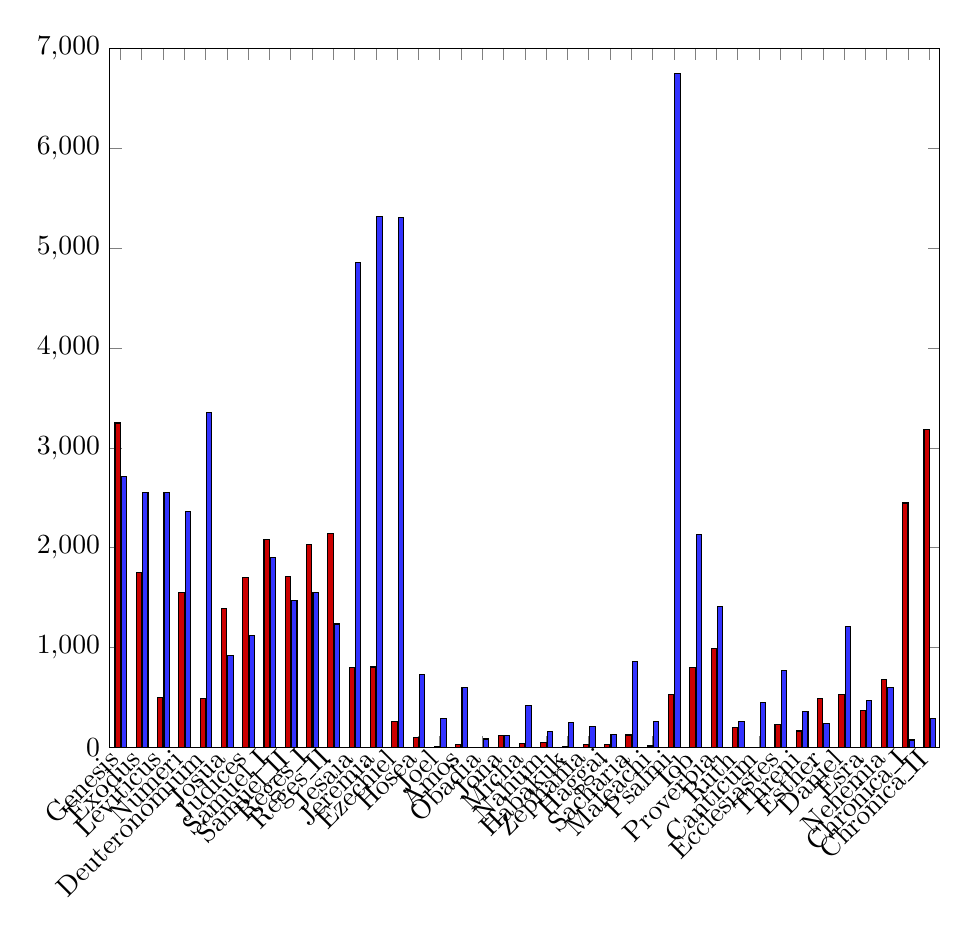
\begin{tikzpicture}[baseline]
\begin{axis}[
width=\textwidth,
xmin=-0.5, xmax=38.5,
ymin=0, ymax=7000,
xtick={0,1,2,3,4,5,6,7,8,9,10,11,12,13,14,15,16,17,18,19,20,21,22,23,24,25,26,27,28,29,30,31,32,33,34,35,36,37,38},
xticklabels={Genesis,Exodus,Leviticus,Numeri,Deuteronomium,Josua,Judices,Samuel\_I,Samuel\_II,Reges\_I,Reges\_II,Jesaia,Jeremia,Ezechiel,Hosea,Joel,Amos,Obadia,Jona,Micha,Nahum,Habakuk,Zephania,Haggai,Sacharia,Maleachi,Psalmi,Iob,Proverbia,Ruth,Canticum,Ecclesiastes,Threni,Esther,Daniel,Esra,Nehemia,Chronica\_I,Chronica\_II},
xticklabel style = {\xticklabel},
]
\draw[draw=\bardrawcolor,fill=\barcolor] (axis cs:-0.25,0) rectangle (axis cs:0,3249);
\draw[draw=\bardrawcolor,fill=\barcolorr] (axis cs:0.05,0) rectangle (axis cs:0.3,2711);
\draw[draw=\bardrawcolor,fill=\barcolor] (axis cs:0.75,0) rectangle (axis cs:1,1750);
\draw[draw=\bardrawcolor,fill=\barcolorr] (axis cs:1.05,0) rectangle (axis cs:1.3,2557);
\draw[draw=\bardrawcolor,fill=\barcolor] (axis cs:1.75,0) rectangle (axis cs:2,501);
\draw[draw=\bardrawcolor,fill=\barcolorr] (axis cs:2.05,0) rectangle (axis cs:2.3,2554);
\draw[draw=\bardrawcolor,fill=\barcolor] (axis cs:2.75,0) rectangle (axis cs:3,1551);
\draw[draw=\bardrawcolor,fill=\barcolorr] (axis cs:3.05,0) rectangle (axis cs:3.3,2359);
\draw[draw=\bardrawcolor,fill=\barcolor] (axis cs:3.75,0) rectangle (axis cs:4,494);
\draw[draw=\bardrawcolor,fill=\barcolorr] (axis cs:4.05,0) rectangle (axis cs:4.3,3351);
\draw[draw=\bardrawcolor,fill=\barcolor] (axis cs:4.75,0) rectangle (axis cs:5,1391);
\draw[draw=\bardrawcolor,fill=\barcolorr] (axis cs:5.05,0) rectangle (axis cs:5.3,925);
\draw[draw=\bardrawcolor,fill=\barcolor] (axis cs:5.75,0) rectangle (axis cs:6,1706);
\draw[draw=\bardrawcolor,fill=\barcolorr] (axis cs:6.05,0) rectangle (axis cs:6.3,1119);
\draw[draw=\bardrawcolor,fill=\barcolor] (axis cs:6.75,0) rectangle (axis cs:7,2086);
\draw[draw=\bardrawcolor,fill=\barcolorr] (axis cs:7.05,0) rectangle (axis cs:7.3,1904);
\draw[draw=\bardrawcolor,fill=\barcolor] (axis cs:7.75,0) rectangle (axis cs:8,1711);
\draw[draw=\bardrawcolor,fill=\barcolorr] (axis cs:8.05,0) rectangle (axis cs:8.3,1469);
\draw[draw=\bardrawcolor,fill=\barcolor] (axis cs:8.75,0) rectangle (axis cs:9,2033);
\draw[draw=\bardrawcolor,fill=\barcolorr] (axis cs:9.05,0) rectangle (axis cs:9.3,1551);
\draw[draw=\bardrawcolor,fill=\barcolor] (axis cs:9.75,0) rectangle (axis cs:10,2144);
\draw[draw=\bardrawcolor,fill=\barcolorr] (axis cs:10.05,0) rectangle (axis cs:10.3,1236);
\draw[draw=\bardrawcolor,fill=\barcolor] (axis cs:10.75,0) rectangle (axis cs:11,801);
\draw[draw=\bardrawcolor,fill=\barcolorr] (axis cs:11.05,0) rectangle (axis cs:11.3,4854);
\draw[draw=\bardrawcolor,fill=\barcolor] (axis cs:11.75,0) rectangle (axis cs:12,805);
\draw[draw=\bardrawcolor,fill=\barcolorr] (axis cs:12.05,0) rectangle (axis cs:12.3,5319);
\draw[draw=\bardrawcolor,fill=\barcolor] (axis cs:12.75,0) rectangle (axis cs:13,257);
\draw[draw=\bardrawcolor,fill=\barcolorr] (axis cs:13.05,0) rectangle (axis cs:13.3,5303);
\draw[draw=\bardrawcolor,fill=\barcolor] (axis cs:13.75,0) rectangle (axis cs:14,96);
\draw[draw=\bardrawcolor,fill=\barcolorr] (axis cs:14.05,0) rectangle (axis cs:14.3,732);
\draw[draw=\bardrawcolor,fill=\barcolor] (axis cs:14.75,0) rectangle (axis cs:15,11);
\draw[draw=\bardrawcolor,fill=\barcolorr] (axis cs:15.05,0) rectangle (axis cs:15.3,292);
\draw[draw=\bardrawcolor,fill=\barcolor] (axis cs:15.75,0) rectangle (axis cs:16,33);
\draw[draw=\bardrawcolor,fill=\barcolorr] (axis cs:16.05,0) rectangle (axis cs:16.3,603);
\draw[draw=\bardrawcolor,fill=\barcolor] (axis cs:16.75,0) rectangle (axis cs:17,1);
\draw[draw=\bardrawcolor,fill=\barcolorr] (axis cs:17.05,0) rectangle (axis cs:17.3,84);
\draw[draw=\bardrawcolor,fill=\barcolor] (axis cs:17.75,0) rectangle (axis cs:18,115);
\draw[draw=\bardrawcolor,fill=\barcolorr] (axis cs:18.05,0) rectangle (axis cs:18.3,116);
\draw[draw=\bardrawcolor,fill=\barcolor] (axis cs:18.75,0) rectangle (axis cs:19,35);
\draw[draw=\bardrawcolor,fill=\barcolorr] (axis cs:19.05,0) rectangle (axis cs:19.3,421);
\draw[draw=\bardrawcolor,fill=\barcolor] (axis cs:19.75,0) rectangle (axis cs:20,47);
\draw[draw=\bardrawcolor,fill=\barcolorr] (axis cs:20.05,0) rectangle (axis cs:20.3,159);
\draw[draw=\bardrawcolor,fill=\barcolor] (axis cs:20.75,0) rectangle (axis cs:21,4);
\draw[draw=\bardrawcolor,fill=\barcolorr] (axis cs:21.05,0) rectangle (axis cs:21.3,250);
\draw[draw=\bardrawcolor,fill=\barcolor] (axis cs:21.75,0) rectangle (axis cs:22,27);
\draw[draw=\bardrawcolor,fill=\barcolorr] (axis cs:22.05,0) rectangle (axis cs:22.3,206);
\draw[draw=\bardrawcolor,fill=\barcolor] (axis cs:22.75,0) rectangle (axis cs:23,25);
\draw[draw=\bardrawcolor,fill=\barcolorr] (axis cs:23.05,0) rectangle (axis cs:23.3,133);
\draw[draw=\bardrawcolor,fill=\barcolor] (axis cs:23.75,0) rectangle (axis cs:24,124);
\draw[draw=\bardrawcolor,fill=\barcolorr] (axis cs:24.05,0) rectangle (axis cs:24.3,861);
\draw[draw=\bardrawcolor,fill=\barcolor] (axis cs:24.75,0) rectangle (axis cs:25,14);
\draw[draw=\bardrawcolor,fill=\barcolorr] (axis cs:25.05,0) rectangle (axis cs:25.3,260);
\draw[draw=\bardrawcolor,fill=\barcolor] (axis cs:25.75,0) rectangle (axis cs:26,529);
\draw[draw=\bardrawcolor,fill=\barcolorr] (axis cs:26.05,0) rectangle (axis cs:26.3,6747);
\draw[draw=\bardrawcolor,fill=\barcolor] (axis cs:26.75,0) rectangle (axis cs:27,800);
\draw[draw=\bardrawcolor,fill=\barcolorr] (axis cs:27.05,0) rectangle (axis cs:27.3,2132);
\draw[draw=\bardrawcolor,fill=\barcolor] (axis cs:27.75,0) rectangle (axis cs:28,991);
\draw[draw=\bardrawcolor,fill=\barcolorr] (axis cs:28.05,0) rectangle (axis cs:28.3,1409);
\draw[draw=\bardrawcolor,fill=\barcolor] (axis cs:28.75,0) rectangle (axis cs:29,199);
\draw[draw=\bardrawcolor,fill=\barcolorr] (axis cs:29.05,0) rectangle (axis cs:29.3,257);
\draw[draw=\bardrawcolor,fill=\barcolor] (axis cs:29.75,0) rectangle (axis cs:30,2);
\draw[draw=\bardrawcolor,fill=\barcolorr] (axis cs:30.05,0) rectangle (axis cs:30.3,454);
\draw[draw=\bardrawcolor,fill=\barcolor] (axis cs:30.75,0) rectangle (axis cs:31,233);
\draw[draw=\bardrawcolor,fill=\barcolorr] (axis cs:31.05,0) rectangle (axis cs:31.3,767);
\draw[draw=\bardrawcolor,fill=\barcolor] (axis cs:31.75,0) rectangle (axis cs:32,164);
\draw[draw=\bardrawcolor,fill=\barcolorr] (axis cs:32.05,0) rectangle (axis cs:32.3,360);
\draw[draw=\bardrawcolor,fill=\barcolor] (axis cs:32.75,0) rectangle (axis cs:33,486);
\draw[draw=\bardrawcolor,fill=\barcolorr] (axis cs:33.05,0) rectangle (axis cs:33.3,241);
\draw[draw=\bardrawcolor,fill=\barcolor] (axis cs:33.75,0) rectangle (axis cs:34,534);
\draw[draw=\bardrawcolor,fill=\barcolorr] (axis cs:34.05,0) rectangle (axis cs:34.3,1212);
\draw[draw=\bardrawcolor,fill=\barcolor] (axis cs:34.75,0) rectangle (axis cs:35,373);
\draw[draw=\bardrawcolor,fill=\barcolorr] (axis cs:35.05,0) rectangle (axis cs:35.3,469);
\draw[draw=\bardrawcolor,fill=\barcolor] (axis cs:35.75,0) rectangle (axis cs:36,683);
\draw[draw=\bardrawcolor,fill=\barcolorr] (axis cs:36.05,0) rectangle (axis cs:36.3,598);
\draw[draw=\bardrawcolor,fill=\barcolor] (axis cs:36.75,0) rectangle (axis cs:37,2448);
\draw[draw=\bardrawcolor,fill=\barcolorr] (axis cs:37.05,0) rectangle (axis cs:37.3,74);
\draw[draw=\bardrawcolor,fill=\barcolor] (axis cs:37.75,0) rectangle (axis cs:38,3184);
\draw[draw=\bardrawcolor,fill=\barcolorr] (axis cs:38.05,0) rectangle (axis cs:38.3,292);
\end{axis}
\end{tikzpicture}


\end{minipage}

\subsection{Narrative, Direct Speech and Quotative Frames}
Direct Speech text portions are part of the text as a whole, but also in a way separate from it: their textual structure is different, the participants and their roles are different, and they are written from different perspectives.

Portions of direct speech usually do not occur out of nowhere; they are introduced by so called \mi{Quotative Frames}, abbreviated as \mi{QF}'s. An important question is the delineation of these \mi{QF}'s and their function in the text. They serve as a bridge between narrative and direct speech, but to what extend do they fit in the text structure of the narrative and to what extend are they dependent on, and influenced by, the content and position of the direct speech portion they are introducing?

It is clear that the options for mentioning speaker and addressee are restricted by the surrounding textual context. When there are three male individuals interacting with each other, for example, a pretty high level of encoding may be necessary to disambiguate who is speaking to whom. When a man and a woman are discussing something, only speech verbs would be enough for disambiguation, because these are inflected for gender. The question remains, however, what is going on beyond this necessary level of identification. To what extent does a narrator play with quotative frames in order to get accross some message about the importance of the quote within the text, or about the social relationship between the participants involved, and so on?

\subsection{The extensiveness of quotative frames}
It is not immediately clear how extensive a quotative frame is, in other words what does belong to the QF and what does not. The \mi{minimal quotative frame} or \mi{quotative frame proper} only contains the clause or clauses with the verb of speech. This verb can be a form of \hebr{>MR}, \hebr{DBR}, or (in \bibleverse{Daniel}) \hebr{MLL}. In the case of \hebr{L>MR} it is reasonable to include the clause immediately preceding \hebr{L>MR} because \hebr{L>MR} is not an independent verb on itself.

Cynthia Miller\autocite{Miller} proposes to include metapragmatic verbs, and thus to make the QF more extensive. Many of these verbs occur with \hebr{L>MR}, and would thus be included in our \mi{minimal quotative frame}, but with less theoretical justification. These verbs are:
%\begin{multicolumn}{2}
    
\begin{itemize}
    \item \hebr{>LH}, `to take an oath'
    \item \hebr{B>R}, `to give news'
    \item \hebr{DJN}, `to argue with'
    \item \hebr{DRC}, `to seek'
    \item \hebr{XNN}, `to implore favor'
    \item \hebr{XRC}, `to be silent'
    \item \hebr{KXC}, `to lie'
    \item \hebr{NB>}, `to prophesy'
    \item \hebr{SWT}, `to incite'
    \item \hebr{<WD}, `to testify'
    \item \hebr{P>R}, `to boast'
    \item \hebr{YXQ}, `to laugh'
    \item \hebr{RMH}, `to deceive'
    \item \hebr{GLH >ZN}, `to uncover ears'
    \item \hebr{HNH DBR JHWH >L}, `behold the word of YHWH was to'
    \item \hebr{HJH DBR JHWH >L}, `the word of YHWH was to'
    \item \hebr{JD<}, `to cause to know'
    \item \hebr{HWYJ> DBH}, `to cause an evil report to go out'
    \item \hebr{MYWT}, `commandments'
    \item \hebr{SPR}, `letter'
    \item \hebr{NTN MWPT}, `to give a sign'
    \item \hebr{<BR HRNH}, `a shout crossed over/through'
    \item \hebr{H<BJR QWL}, `to cause the sound to cross over'
    \item \hebr{FJM <LJLT DBRJM}, `to make baseless charges'
\end{itemize}

%\end{multicolumn}

Other metapragmatical verbs occur (also) with a finite form of \hebr{>MR}, and sometimes they are the only verb of speech present. The verbs for which this holds, and that would thus not be included when using the minimal definition of QF, are:
%\begin{multicolumn}{2}
Occurring as single speech verb:
\begin{itemize}
\item \hebr{SPD}, `to mourn'
\item \hebr{<NH}, `to answer'
\item \hebr{QR>}, `to call'
\item \hebr{Z<Q}, `to cry out'
\item \hebr{NGD}, `to tell'
\item \hebr{YWH}, `to command'
\item \hebr{Y<Q}, `to cry out'
\item \hebr{C>L}, `to ask/greet'
\item \hebr{CB<}, `to swear'
\item \hebr{CLX}, `to send'
\item \hebr{KTB}, `to write'
\item \hebr{CM<}, `to hear'
\item \hebr{CJD}, `to sing'
\end{itemize}
Not occurring as single speech verb:
\begin{itemize}
\item \hebr{BRK}, `to bless'
\item \hebr{NDR}, `to vow'
\item \hebr{SPR}, `to recount'
\item \hebr{PLL}, `to pray'
\item \hebr{HTL}, `to mock'
\item \hebr{QLS}, `to mock'
\item \hebr{M>N}, `to refuse'
\item \hebr{NXM}, `to comfort'
\item \hebr{QWN} or \hebr{QJN}, `to lament'
\item \hebr{<TR}, `to pray'
\item \hebr{RW<}, `to give a shout'
\item \hebr{FJM DBR}, `to put a word'
\item \hebr{HJH MCL}, `a proverb was'
\item \hebr{NF> MC>}, `to raise a proverb'
\item \hebr{HRJM QWL}, `to cause a shout to rise'
\item \hebr{BKH}, `to weep'
\item \hebr{HCJB DBR}, `cause a word to return'
\item \hebr{J<Y}, `to take counsel'
\item \hebr{XRP}, `to reproach'
\item \hebr{LWN}, `to grumble'
\item \hebr{RJB}, `to strive, contend'
\item \hebr{TQ<}, `to sound the ram's horn'
\end{itemize}
%\end{multicolumn}

\autocite[210-212]{Miller}

Just the occurrence of one of those verbs does not make it part of the quotative frame. There are some further restrictions: ``each verb refers to the same speech event, the speech participants are identical and have identical roles, the verbs share arguments, the verbs are inflected identically with respect to gender and number (with corporate entities this may be different), and the tense/aspect is either identical or consecutive.'' \autocite[204-205]{Miller} If I understand Miller correctly, a sequence of multiple metapragmatic verbs can form a pretty extensive quotative frame, as for example in \bibleverse{Gen}(28:01): \hebr{\cl{red}{W JQR>} JYXQ >L J<QB \cl{red}{W JBRK} >TW \cl{red}{W JYWHW} \cl{red}{W J>MR} LW}.

Miller's theory is an adaptation of an even more elaborate proposal made by Longacre. \autocite{Longacre}. He proposes to include verbs of motion, psychological verbs, and metapragmatic verbs, which in some cases means that ``the clause with the verb `say' may be preceded by two or three such preparatory clauses. In such a situation the whole sequence of two to four clauses with whatever nouns and pronouns that it contains is relevant to the specification or nonspecification of speaker and addressee; it functions as an \emph{expanded quotation formula}.'' \autocite[160]{Longacre}
This very extensive view of quotative frames makes the boundary between QF and surrounding narrative less strict; the QF is more a fluent part of the narrative that just happens to be positioned before the direct speech section, instead of a separate block in between the narrative and the quote. 
At the very least, as Miller notes \autocite[204-205]{Miller}, Longacre's theory does not make very clear when a clause does or does not belong to the quotative frame.

\subsection{Perspective and information}
Direct speech sections are spoken by a speaker, in principle from his own perspective. This perspective might differ from that of the narrator and the reader. In some cases it is clear that the speaker lacks information that the reader has, for example in \bibleverse{Gen}(27:18), where Isaak asks \hebr{MJ >TH BNJ}, and the narrator has told already about Jacob's plans to deceive his father.

Since direct speech portions reflect the perspective of the speaker and addressee, participant references in these portions are chosen from their perspective as well.

The reverse is also true, namely that speakers and addressees have a corpus of knowledge that readers do not share. It is the narrator's task to make their conversations intelligible for readers by selecting quotes, narrating background stories et cetera. But this is never done ``objectively'', as if every possible narrator would do this in exactly the same way. Narrators have a purpose with their stories; they select and arrange the narrated information accordingly. This process of arrangement is, among other ways, reflected in the framing of direct speech sections.

\subsection{Basic rules for participant encoding in direct speech}
Runge \autocite{Runge} described a basic system for participant references in narrative texts. Using a similar model for direct speech texts asks for some extra rules:
\begin{itemize}
    \item Speaker and addressee, in first and second person respectively, are active participants. They need not be introduced by a noun or personal name, for the speech setting alone is sufficient for disambiguation.
    \item The identification of speaker and addressee for the \emph{reader} happens in the quotative frame, not in the direct speech section itself. The direct speech section is encoded from the perspective of the interlocutors, not from that of the narrator or reader.
    \item Honorifics and other complex forms denoting speaker and addressee are, \emph{with respect to their identity}, equated with straightforward first and second person denotations. (It is clear that the marked formulation used has to be accounted for in other aspects of our analysis.) In other words, expressions like \hebr{NPCK} (e.g. \bibleverse{Gen}(27:19)) semantically have the same value as a simple "you". This is important for the encoding of following references to the same person, that thus do not need to be overencoded as if there had been a switch of referent, and for references to other persons, that might be ambiguous if the honorific form would be seen as a third person reference. An example to clarify this is found in \bibleverse{Gen}(6:3), where JHWH says: \hebr{L> JDWN \cl{red}{RWXJ} B H >DM L <WLM B C GM \cl{red}{HJW} BFR}. In the first clause, \hebr{RWXJ} is subject. In the subordinated clause that follows, the \hebr{>DM} is subject, and only encoded with a personal pronoun. My hypothesis is that this is possible because \hebr{RWXJ} is not seen as a third person masculine, but as a first person. 
\end{itemize}

\subsection{Some constraints on encoding options}

\section{Observations from computer-assisted analyses}
\section{Model of participant reference system}
\newpage
\section{Conclusion}
\subsection{Research results}
\subsection{Areas for further research}
\subsection{Conclusion}
\newpage
\section*{Bibliography}
\printbibliography

\end{document}




Miller [204-205]: When a quotative frame has multiple finite metapragmatic verbs (note: Longacre includes motion verbs and psychological verbs, but Miller includes only metapragmatic verbs within the quotative frame --> boundaries clear), each verb refers to the same speech event, the speech participants are identical and have identical roles, | the verbs share arguments, the verbs are inflected identically with respect to gender and number (with corporate entities this may be different), and the tense/aspect is either identical or consecutive.


[160]
``Quotation formulas \emph{proper} consist of some form of the verb'' >MR ``+/- nouns and/or
pronouns. Very frequently, however, the clause that contains the verb `say' is preceded by another clause that has either a \emph{motion} verb (`and they drew near to him, and they said'); a verb of \emph{psychological} orientation (`and they feared greatly, and they said'); or a \emph{verb} that is more specific in relation to the speech act (`and he refused, and he said'). Furthermore, the clause with the verb `say' may be preceded by two or three such preparatory clauses. In such a situation the whole sequence of two to four clauses with whatever nouns and pronouns that it contains is relevant to the specification or nonspecification of speaker and addressee; it functions as an \emph{expanded quotation formula}.''

Longacre sees no difference between nouns etc in preceding clauses and those in the quotation formula proper.

